\documentclass[10pt,twocolumn]{article}
\usepackage[utf8]{inputenc}
\usepackage[T1]{fontenc}
\usepackage{lmodern}
\usepackage{amsmath,amssymb}
\usepackage{graphicx}
\usepackage{booktabs}
% --- reemplazo minimo de siunitx (no instalado) ---
\providecommand{\SI}[2]{#1\,#2}
\providecommand{\SIrange}[3]{#1--#2\,#3}
\providecommand{\si}[1]{#1}
\providecommand{\meter}{m}\providecommand{\milli}{m}\providecommand{\kilo}{k}
\providecommand{\gram}{g}\providecommand{\newton}{N}\providecommand{\hertz}{Hz}
\providecommand{\per}{/}\providecommand{\degree}{\ensuremath{^\circ}}
\usepackage[margin=1.8cm]{geometry}
\usepackage{float}
\usepackage[hidelinks]{hyperref}
\usepackage{caption}
\captionsetup{font=small}
\usepackage{listings}
\lstset{basicstyle=\ttfamily\scriptsize,breaklines=true,columns=fullflexible,
  keepspaces=true,showstringspaces=false,frame=single,xleftmargin=3pt,aboveskip=4pt,belowskip=2pt}

\title{\textbf{OpenOmni}: dise\~no e ingenier\'ia de una cinta omnidireccional
pasiva de realidad virtual, imprimible en 3D y de bajo costo}
\author{Nicol\'as \'Alvarez}
\date{\today}

\begin{document}
\maketitle

\begin{abstract}
\noindent
OpenOmni es una plataforma de locomoci\'on omnidireccional \emph{pasiva} para realidad
virtual (VR), concebida como una r\'eplica funcional y econ\'omica del \emph{Virtuix
Omni One}, construible con madera, tubo de acero, componentes de bicicleta, un resorte
de gas y piezas impresas en 3D. El sistema resuelve el conflicto vestibular de la VR
permitiendo caminar y correr f\'isicamente en el sitio: un cuenco c\'oncavo de baja
fricci\'on recentra el pie por gravedad, mientras un brazo articulado posterior --montado
como una mochila y girando \SI{360}{\degree} sobre un rodamiento central-- sostiene al
usuario. Este documento presenta la biomec\'anica del cuenco, la cinem\'atica del brazo
mediante par\'ametros de Denavit--Hartenberg, la f\'isica del muelle neum\'atico, el
an\'alisis de fuerzas y estabilidad, la estructura mec\'anica, y la electr\'onica de
seguimiento inercial de los pies. Se incluye un \emph{gemelo digital} interactivo
(Three.js) que valida la geometr\'ia y visualiza las fuerzas en vivo.
\end{abstract}

\section{Introducci\'on}
La locomoci\'on ha sido el problema abierto de la VR durante m\'as de una d\'ecada: el
conflicto entre el sistema visual (que percibe movimiento) y el vestibular (que permanece
est\'atico) provoca cinetosis. Las cintas omnidireccionales resuelven el conflicto
haciendo que el usuario camine realmente. El \emph{Virtuix Omni One} es el referente
comercial: una base c\'oncava de baja fricci\'on m\'as un brazo de soporte que reemplaza
al aro de contenci\'on de generaciones previas. Su costo (US\$2.600--3.500) motiva este
trabajo: \textbf{OpenOmni} reproduce sus principios con un presupuesto de
US\$250--430 usando materiales de ferreter\'ia e impresi\'on 3D.

El sistema es \emph{pasivo}: no emplea motores para la locomoci\'on ni para el soporte.
La gravedad y la geometr\'ia hacen el trabajo. Esto simplifica dr\'asticamente la
construcci\'on y elimina la seguridad funcional asociada a actuadores.

\section{Arquitectura del sistema}
OpenOmni se compone de seis subsistemas (Fig.~\ref{fig:webui}):
\begin{enumerate}\itemsep2pt
  \item \textbf{Cuenco c\'oncavo} ($\varnothing$\SI{1.2}{\meter}, pendiente de borde
  \SI{13}{\degree}): superficie parab\'olica de baja fricci\'on.
  \item \textbf{Estructura}: oct\'agono de madera sobre patas, con lastre anti-vuelco.
  \item \textbf{Brazo articulado + arn\'es}: 3 GDL pasivos, girando \SI{360}{\degree}
  sobre un rodamiento central.
  \item \textbf{Sistema hidr\'aulico}: resorte de gas que soporta la carga vertical.
  \item \textbf{Calzado deslizante}: sobre-zapatos con almohadillas de PTFE/UHMW.
  \item \textbf{Electr\'onica}: sensores inerciales en los pies (estilo SlimeVR) que se
  presentan al PC como un mando USB.
\end{enumerate}

\begin{figure}[H]
\centering
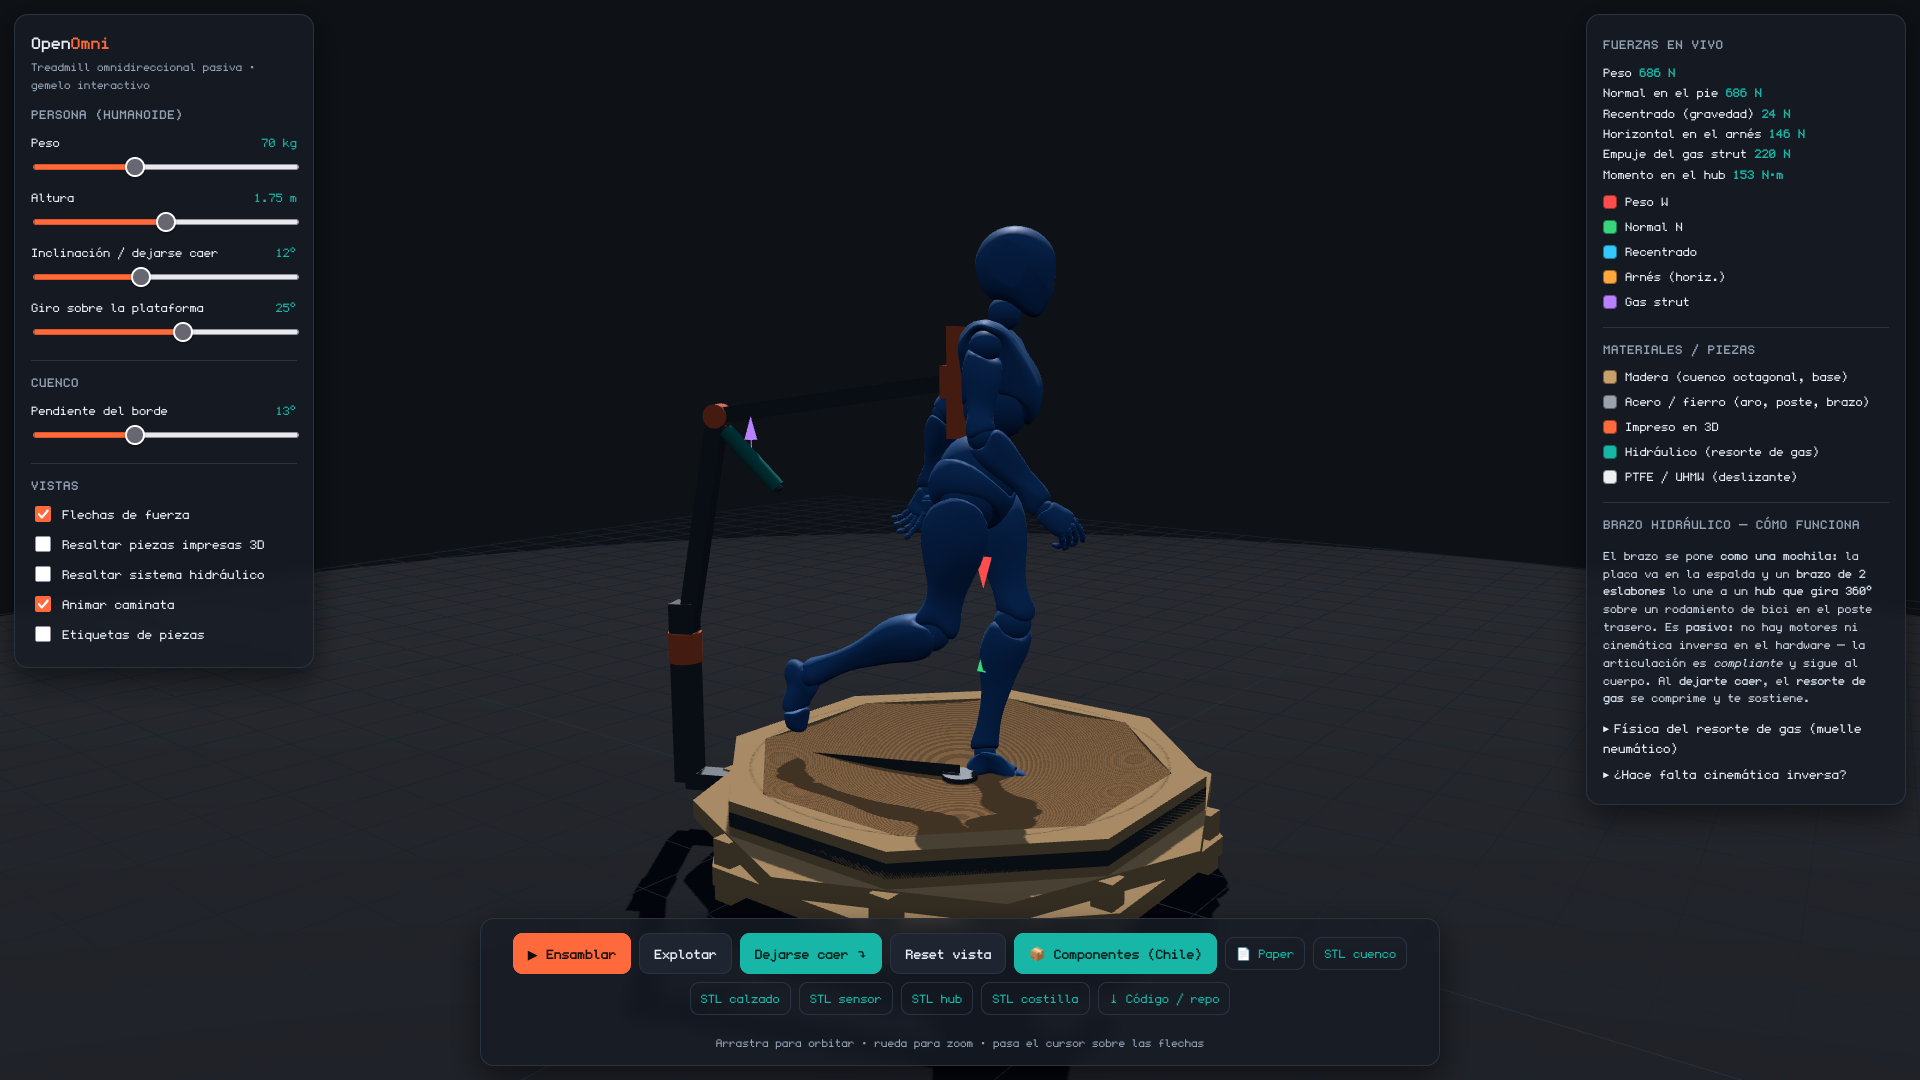
\includegraphics[width=\linewidth]{fig_webui.png}
\caption{Gemelo digital interactivo de OpenOmni (Three.js). El maniqu\'i (\SI{70}{\kilo\gram})
camina en el cuenco octagonal; el brazo posterior tipo mochila y su resorte de gas
aparecen a la izquierda. Las flechas representan las fuerzas en vivo.}
\label{fig:webui}
\end{figure}

\section{Cuenco c\'oncavo: geometr\'ia y biomec\'anica}
La superficie sigue un perfil parab\'olico de revoluci\'on
\begin{equation}
z(r) = k\,r^{2}, \qquad k=\frac{\tan\theta_{b}}{2R},
\end{equation}
con radio $R=\SI{0.6}{\meter}$ y pendiente de borde $\theta_b=\SI{13}{\degree}$, de donde
$k=\SI{1.924e-4}{\per\milli\meter}$ y una profundidad central de \SI{69}{\milli\meter}.

En el radio $r$, la pendiente local es $\tan\theta(r)=2kr$. El peso del pie apoyado
$W_p$ (hasta el peso corporal $W$ en apoyo monopodal) se descompone en una normal
$N=W_p\cos\theta$ y una componente tangencial de \emph{recentrado}
\begin{equation}
F_{\text{rec}} = W_p\,\sin\theta(r),
\end{equation}
que devuelve el pie al centro. Para que el pie deslice de vuelta (y no se quede pegado)
se requiere $F_{\text{rec}}>\mu N$, es decir
\begin{equation}
\boxed{\ \tan\theta(r) > \mu\ }
\end{equation}
Con un coeficiente de fricci\'on objetivo $\mu\approx0.10$ (PTFE/UHMW con lubricante de
silicona), el pie se auto-recentra para $r\gtrsim\SI{0.26}{\meter}$. El compromiso es
fino: una pendiente mayor fatiga el tibial (\SI{250}{\newton} por paso en el borde para
$W=\SI{1110}{\newton}$), mientras que una menor deja al usuario derivar contra el arn\'es.
La ingenier\'ia de fricci\'on ($\mu<0.12$) es el requisito de dise\~no primario.

\section{Cinem\'atica del brazo de soporte}
El brazo es una cadena serial de 3 GDL desde un rodamiento central hasta el punto de la
mochila en la espalda (Fig.~\ref{fig:bearing}). Sus par\'ametros de
Denavit--Hartenberg (est\'andar) se listan en la Tabla~\ref{tab:dh}.

\begin{table}[H]
\centering
\begin{tabular}{ccccc}
\toprule
$i$ & articulaci\'on & $a_i$ & $\alpha_i$ & $d_i$ \\
\midrule
1 & giro (yaw) & $a_1$ & \SI{90}{\degree} & $d_1$ \\
2 & hombro     & $L_1$ & \SI{0}{\degree}  & $0$ \\
3 & codo       & $L_2$ & \SI{0}{\degree}  & $0$ \\
\bottomrule
\end{tabular}
\caption{Par\'ametros DH del brazo. $\theta_1$ (giro sobre la plataforma) sigue al usuario;
$a_1$ es el brazo radial del centro al poste; $d_1$ la altura del hombro; $L_1,L_2$ los
eslabones ($=\SI{0.7}{\meter}$).}
\label{tab:dh}
\end{table}

La matriz homog\'enea de cada eslabón es
\begin{equation}
{}^{i-1}\!A_i=
\begin{bmatrix}
c_{\theta_i} & -s_{\theta_i}c_{\alpha_i} & s_{\theta_i}s_{\alpha_i} & a_i c_{\theta_i}\\
s_{\theta_i} &  c_{\theta_i}c_{\alpha_i} & -c_{\theta_i}s_{\alpha_i} & a_i s_{\theta_i}\\
0 & s_{\alpha_i} & c_{\alpha_i} & d_i\\
0&0&0&1
\end{bmatrix},
\end{equation}
y la pose del efector final (chaleco) es
$\,{}^{0}T_3={}^{0}\!A_1\,{}^{1}\!A_2\,{}^{2}\!A_3$.

\paragraph{Naturaleza pasiva.} En el hardware \emph{no hay actuadores ni cinem\'atica
inversa}: las tres articulaciones son de revoluci\'on libres (rodamientos) y el resorte
de gas provee compliancia en el eje vertical. El brazo sigue al cuerpo por pura mec\'anica,
como una l\'ampara de brazo articulado. El giro $\theta_1$ mantiene el brazo detr\'as del
usuario al rotar \SI{360}{\degree}.

\paragraph{Gemelo digital.} Para \emph{dibujar} el brazo persiguiendo la espalda (que se
mueve con la altura, el giro y la inclinaci\'on), el simulador s\'i resuelve la cinem\'atica
inversa planar de 2 eslabones. Dado el objetivo $(p_x,p_y)$ en el plano del brazo y su
alcance $D=\sqrt{p_x^2+p_y^2}$,
\begin{align}
\cos\theta_3 &= \frac{D^2-L_1^2-L_2^2}{2L_1L_2},\\
\theta_2 &= \operatorname{atan2}(p_y,p_x) + \arccos\!\frac{D^2+L_1^2-L_2^2}{2L_1D}.
\end{align}

\section{Sistema hidr\'aulico: el resorte de gas}
El soporte vertical lo provee un \emph{muelle neum\'atico} (gas strut): un pist\'on
encierra nitr\'ogeno a presi\'on $P_0$ (Fig.~\ref{fig:strut}). Al comprimir el v\'astago
una distancia $x$, el volumen disminuye y, en un proceso casi adiab\'atico,
\begin{equation}
P\,V^{\gamma}=\text{const},\qquad \gamma\approx1.4,
\end{equation}
por lo que la fuerza de soporte
\begin{equation}
F(x)=P(x)\,A_{\text{ef}},\quad
P(x)=P_0\!\left(\frac{V_0}{V_0-A_{\text{ef}}\,x}\right)^{\!\gamma}
\end{equation}
crece con la compresi\'on: el muelle es \emph{progresivo} (auto-limita la ca\'ida). El
sellado con aceite a\~nade amortiguaci\'on viscosa $F_d=c\,\dot{x}$, eliminando el rebote.

\paragraph{Acoplamiento con el brazo.} El strut se monta como \emph{puente del codo}: un
extremo en el eslab\'on inferior a distancia $a$ del codo, el otro en el superior a
distancia $b$. Su longitud queda ligada al \'angulo interior del codo $\varphi$ por la
ley de cosenos
\begin{equation}
\boxed{\ L_s^2 = a^2 + b^2 - 2ab\cos\varphi\ }
\end{equation}
As\'i, al agacharse o dejarse caer, el codo se cierra ($\varphi$ disminuye), el strut se
comprime y la fuerza progresiva sostiene al usuario. El dimensionado nominal
($F\approx0.32\,W\approx\SI{350}{\newton}$, carrera $\geq\SI{120}{\milli\meter}$) se cubre
con un cilindro de silla de oficina o un amortiguador de port\'on.

\begin{figure}[H]
\centering
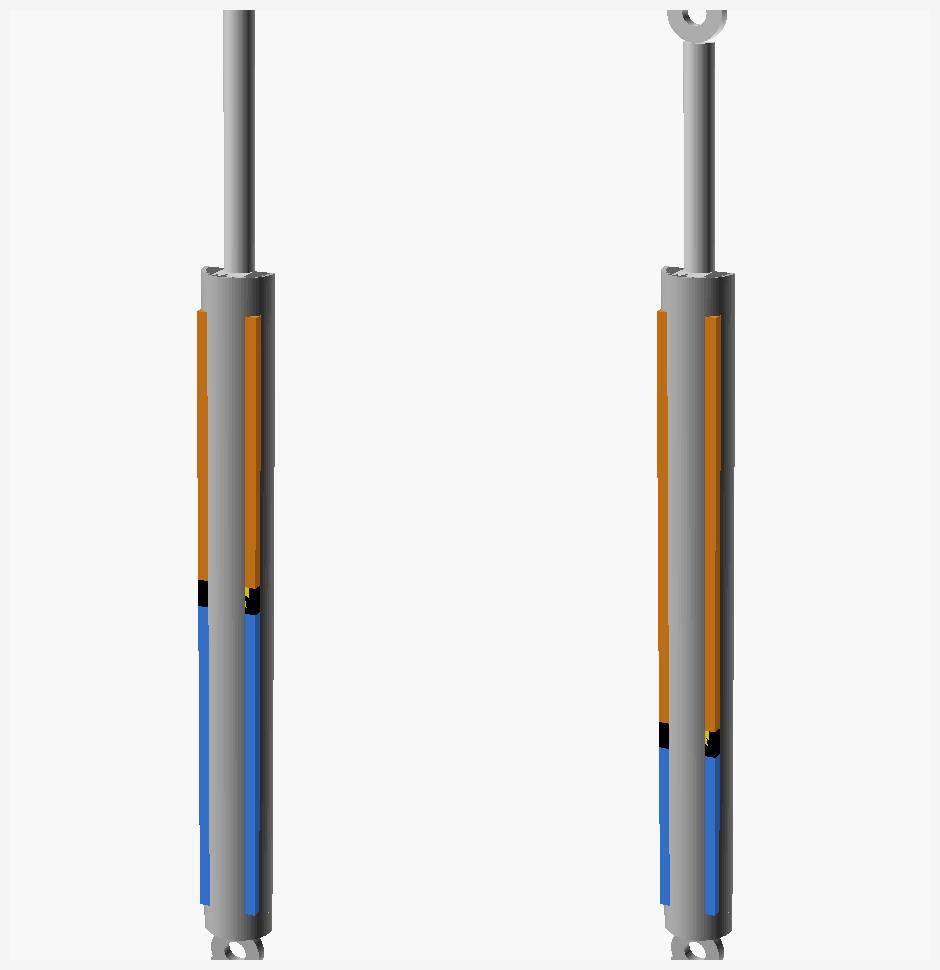
\includegraphics[width=\linewidth]{fig_strut.png}
\caption{Corte del resorte de gas modelado en OpenSCAD (extendido vs.\ comprimido):
c\'amara de gas N$_2$ (azul), aceite de amortiguaci\'on (\'ambar), pist\'on y v\'astago.}
\label{fig:strut}
\end{figure}

\section{Fuerzas y estabilidad}
Modelando al usuario como p\'endulo invertido apoyado en los pies y sostenido atr\'as por
el brazo, la fuerza horizontal en el arn\'es al inclinarse un \'angulo $\phi$ es
$P_h=W\tan\phi$ (hasta $\sim\SI{600}{\newton}$ en sprint). El momento en el rodamiento del
hub $M=P_h\,h_v\approx\SI{630}{\newton\meter}$ debe reaccionarse como par de fuerzas
(dos rodamientos separados) o con un rodamiento de momento (rueda de remolque).

\paragraph{Vuelco.} El momento de vuelco $M_v=P_h h_v$ es cr\'itico durante un salto
(cuando el peso del usuario desaparece). La soluci\'on --como en el Omni One, que pesa
\SI{70}{\kilo\gram} a prop\'osito-- es \textbf{lastrar la base} con
\SI{25}{}--\SI{30}{\kilo\gram} (arena/concreto) para un factor de seguridad
$\geq2$ sin depender del usuario.

\section{Estructura mec\'anica y juntas}
La base es un \textbf{oct\'agono de ocho m\'odulos} de madera (siguiendo el patr\'on de
vigas radiales tipo rayos + bloque central + deck de terciado laminado). Las uniones
cr\'iticas radial--centro se ejecutan con \emph{tornillos estructurales} \SI{8x80}{\milli\meter}
m\'as adhesivo D3 (no s\'olo clavos). El giro emplea \textbf{un rodamiento central} (rueda
de remolque o plato giratorio), muy superior a un ra\'il perimetral en facilidad y suavidad.

\paragraph{Juntas impresas en 3D.} Las abrazaderas impresas act\'uan como
\emph{locator/clamp}: la carga real la toma un \textbf{perno de acero pasante}
(Fig.~\ref{fig:mount}), nunca el pl\'astico. Los alojamientos de tubo se dise\~nan con
$\SI{+0.4}{\milli\meter}$ de tolerancia (FDM), pared $\geq\SI{4}{\milli\meter}$ e inserto
roscado met\'alico para el apriete.

\begin{figure}[H]
\centering
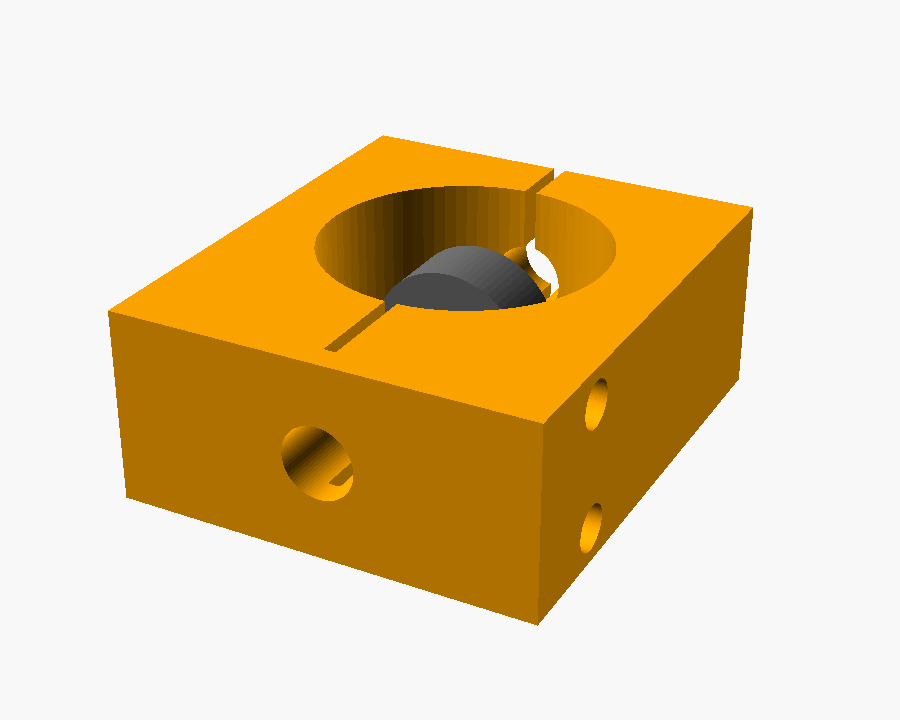
\includegraphics[width=0.8\linewidth]{fig_mount.png}
\caption{Junta realista (OpenSCAD): abrazadera impresa (naranja) con alojamiento de tubo,
ranura de \emph{split-clamp}, pernos M5 y \textbf{perno M8 pasante} de acero que soporta la
carga; el ojal de acero del strut se monta en ese perno.}
\label{fig:mount}
\end{figure}

\section{Electr\'onica y firmware}
Cada pie lleva un microcontrolador ESP32-C3 con una IMU de 9 ejes (MPU-9250) y un sensor
de presi\'on (FSR) en el tal\'on. La orientaci\'on se estima con un filtro de Mahony a
\SI{200}{\hertz}; la aceleraci\'on lineal se integra con \emph{ZUPT} (zero-velocity update)
para estimar la velocidad de deslizamiento del pie. Los datos viajan por ESP-NOW a un hub
ESP32-S3 que fusiona el vector de locomoci\'on --con \emph{desacople de rumbo}: la
direcci\'on proviene de los pies, no de la cabeza-- y se presenta al PC como un
\textbf{mando USB HID}, funcionando en SteamVR y cualquier juego sin drivers propietarios.

\section{Gemelo digital interactivo}
Todo el dise\~no se valida en un gemelo digital web (Three.js) desplegado en GitHub Pages
(Fig.~\ref{fig:bearing}). Permite variar peso (\SIrange{40}{120}{\kilo\gram}) y altura
(\SIrange{1.5}{2.0}{\meter}) del maniqu\'i, inclinarlo, girarlo y ensamblarlo/explotarlo,
mostrando las fuerzas en vivo y un panel de componentes con enlaces de compra. Sirve como
herramienta de dise\~no y de comunicaci\'on del sistema.

\begin{figure}[H]
\centering
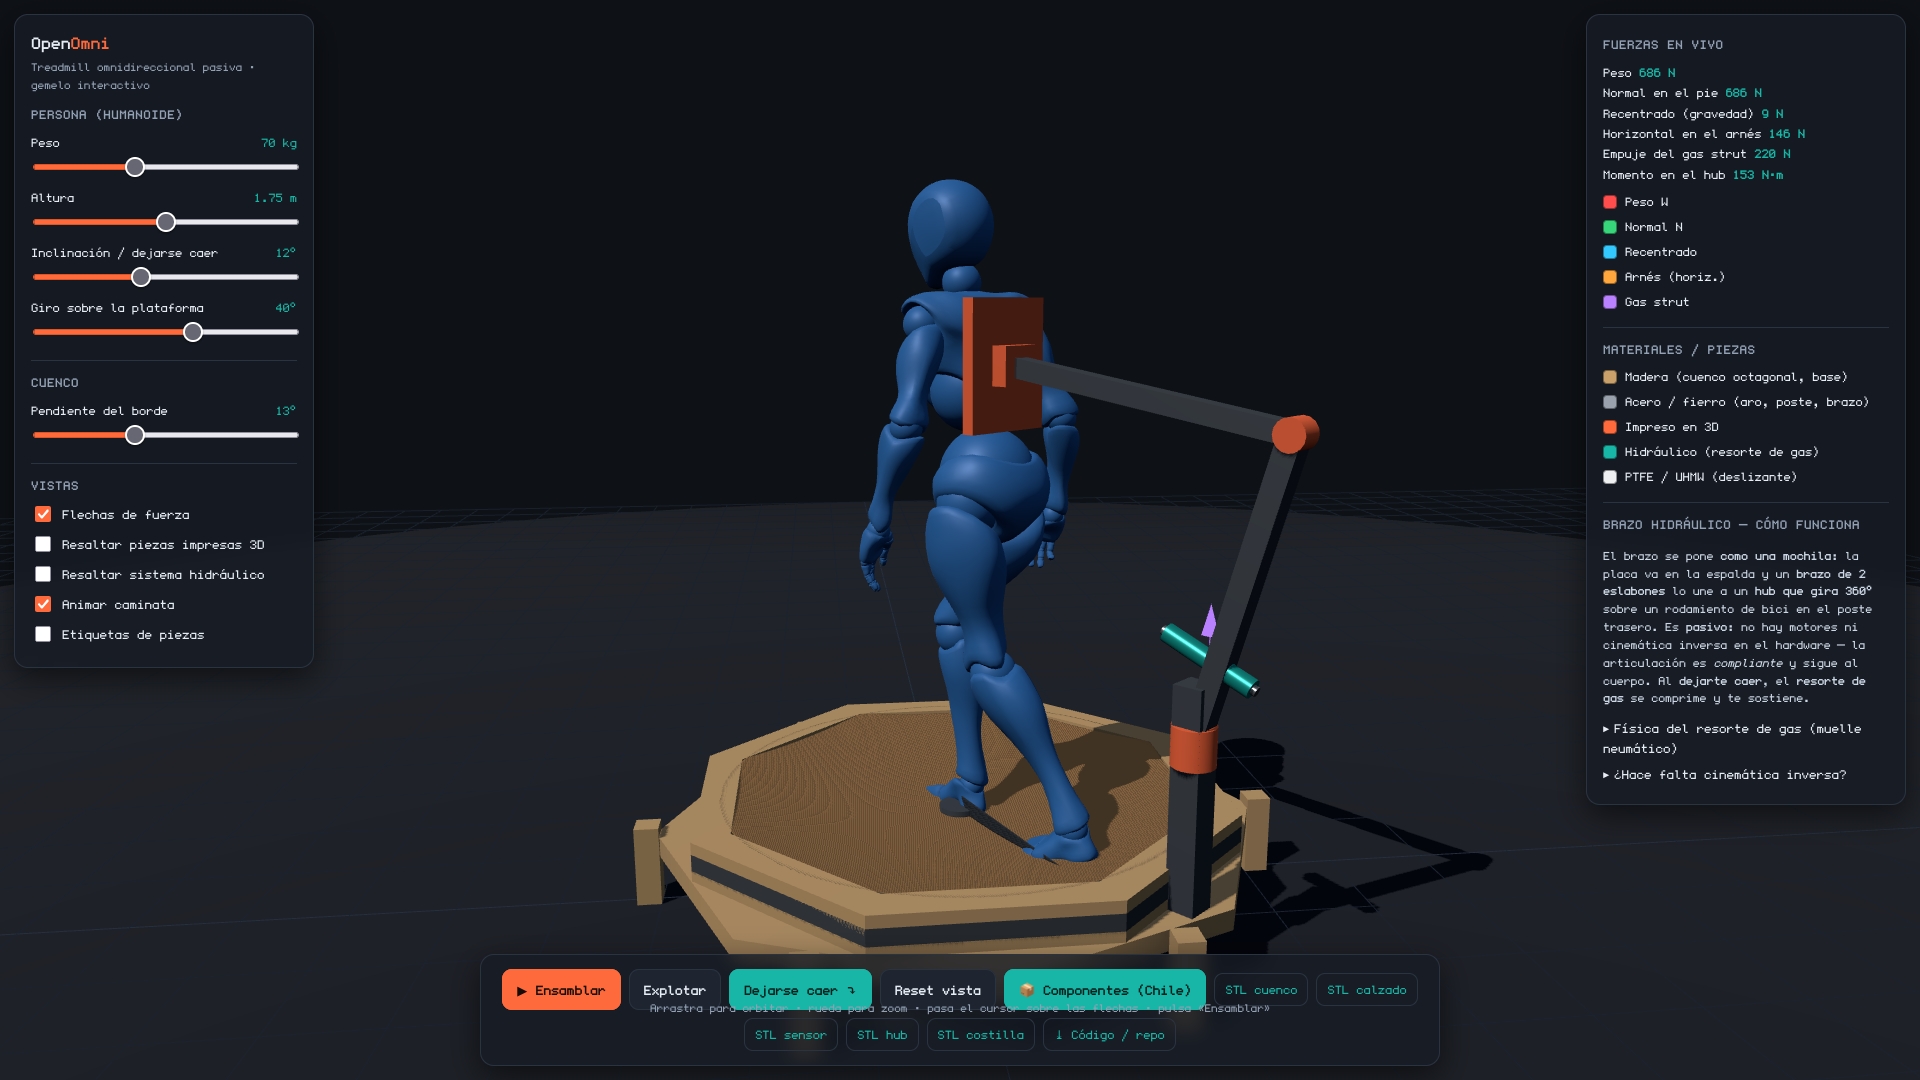
\includegraphics[width=\linewidth]{fig_bearing.png}
\caption{Plataforma elevada sobre patas: el mecanismo de giro (rodamiento central + brazo
radial + poste) queda visible en el hueco inferior.}
\label{fig:bearing}
\end{figure}

\section{Conclusiones}
OpenOmni demuestra que los principios del Omni One --cuenco parab\'olico de baja fricci\'on
con recentrado gravitacional, brazo articulado compliante y seguimiento inercial-- son
reproducibles con materiales de ferreter\'ia e impresi\'on 3D a $\sim$1/8 del costo. Los
puntos cr\'iticos son la fricci\'on del cuenco ($\mu<0.12$), el lastre anti-vuelco y el uso
de acero (no pl\'astico) en las juntas cargadas. El gemelo digital y los modelos
param\'etricos (OpenSCAD) hacen el dise\~no auditable y modificable.

\onecolumn
\section{Ap\'endice: firmware del tracker de pie (extracto)}
El c\'odigo completo est\'a en \texttt{firmware/foot\_tracker/}. Se muestran el filtro de
Mahony (fusi\'on de aceler\'ometro + giroscopio a cuaterni\'on) y el bucle principal, que
integra la aceleraci\'on lineal con \emph{ZUPT} y obtiene la velocidad de deslizamiento
del pie hacia atr\'as --la se\~nal de ``caminar''-- enviada por ESP-NOW al hub.

\begin{lstlisting}[language=C++]
void mahonyUpdate(float gx,float gy,float gz,float ax,float ay,float az,float dt){
    float recipNorm;
    float halfvx,halfvy,halfvz;
    float halfex,halfey,halfez;

    if(!(ax==0 && ay==0 && az==0)){
        recipNorm = 1.0f/sqrtf(ax*ax+ay*ay+az*az); ax*=recipNorm; ay*=recipNorm; az*=recipNorm;
        // gravedad estimada desde el quaternion
        halfvx = q1*q3 - q0*q2;
        halfvy = q0*q1 + q2*q3;
        halfvz = q0*q0 - 0.5f + q3*q3;
        // error = producto cruz medido x estimado
        halfex = (ay*halfvz - az*halfvy);
        halfey = (az*halfvx - ax*halfvz);
        halfez = (ax*halfvy - ay*halfvx);
        if(twoKi>0.0f){
            integralFBx += twoKi*halfex*dt; integralFBy += twoKi*halfey*dt; integralFBz += twoKi*halfez*dt;
            gx += integralFBx; gy += integralFBy; gz += integralFBz;
        }
        gx += twoKp*halfex; gy += twoKp*halfey; gz += twoKp*halfez;
    }
    // integra el rate de giro
    gx*=0.5f*dt; gy*=0.5f*dt; gz*=0.5f*dt;
    float qa=q0, qb=q1, qc=q2;
    q0 += (-qb*gx - qc*gy - q3*gz);
    q1 += ( qa*gx + qc*gz - q3*gy);
    q2 += ( qa*gy - qb*gz + q3*gx);
    q3 += ( qa*gz + qb*gy - qc*gx);
    recipNorm = 1.0f/sqrtf(q0*q0+q1*q1+q2*q2+q3*q3);
    q0*=recipNorm; q1*=recipNorm; q2*=recipNorm; q3*=recipNorm;
}

void loop(){
    uint32_t now=micros();
    float dt=(lastMicros==0)?0.005f:(now-lastMicros)*1e-6f; lastMicros=now;
    if(dt<=0 || dt>0.1f) dt=0.005f;

    float ax,ay,az,gx,gy,gz;
    imuRead(ax,ay,az,gx,gy,gz);
    mahonyUpdate(gx,gy,gz,ax,ay,az,dt);

    // aceleracion lineal en el mundo (quita la gravedad)
    float wx,wy,wz; bodyAccelToWorld(ax,ay,az,wx,wy,wz);
    wx*=G; wy*=G; wz=(wz-1.0f)*G;               // resta 1g en Z-mundo
    float amag=sqrtf(wx*wx+wy*wy);

    int fsr=analogRead(PIN_FSR);
    bool contact = fsr > 400;                    // FSR: contacto con el cuenco

    velX += wx*dt; velY += wy*dt;                // integra velocidad horizontal

    // ZUPT: contacto + poca aceleracion => pie quieto => resetea deriva
    if(contact && amag < 0.6f){
        if(millis()-lastZupt > 40){ velX*=0.5f; velY*=0.5f; }
    } else { lastZupt=millis(); }
    velX*=0.995f; velY*=0.995f;                  // fuga lenta anti-runaway

    // rumbo del pie y velocidad de deslizamiento HACIA ATRAS = caminar
    float yaw=yawDeg();
    float fwdx=cosf(yaw*DEG_TO_RAD), fwdy=sinf(yaw*DEG_TO_RAD);
    float vForward = velX*fwdx + velY*fwdy;
    float backSpeed = (vForward < 0) ? -vForward : 0.0f;
    backSpeed = constrain(backSpeed, 0.0f, 3.5f);

    if(millis()-lastTx >= 10){                   // envia a 100 Hz por ESP-NOW
        lastTx=millis();
        sendPacket(yaw, contact?backSpeed:0.0f, contact?1:0);
    }
}
\end{lstlisting}

\begin{thebibliography}{9}
\small
\bibitem{virtuix} Virtuix, \emph{Omni One} --- documentaci\'on t\'ecnica y patentes
(US 20230356099 A1; US 11,247,126).
\bibitem{slimevr} SlimeVR, \emph{SlimeVR-Tracker-ESP}, seguimiento inercial de c\'odigo abierto.
\bibitem{woodt} \emph{WoODT --- Wooden Omni Directional Treadmill}, movesilently.de.
\bibitem{mahony} R.\ Mahony et al., ``Nonlinear complementary filters on the special
orthogonal group,'' \emph{IEEE Trans.\ Automatic Control}, 2008.
\bibitem{craig} J.\ J.\ Craig, \emph{Introduction to Robotics: Mechanics and Control},
par\'ametros de Denavit--Hartenberg.
\end{thebibliography}

\end{document}
